\section*{Problem 4}
\begin{enumerate}
\item For the principal component regression models the plots of training error v.s. number of components and test error v.s. number of principal components are below, respectively. Based on the training data, 8 components would be best, while 7 or possibly 3 components could produce comparable results. The test data suggests that 5 or 6 components would be best, and 8 components could produce comparable results.  \newline 
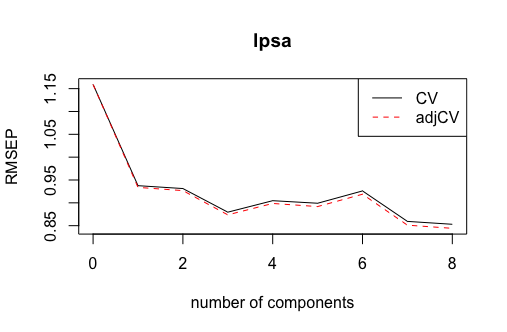
\includegraphics[width=\textwidth]{img/pcr.png}
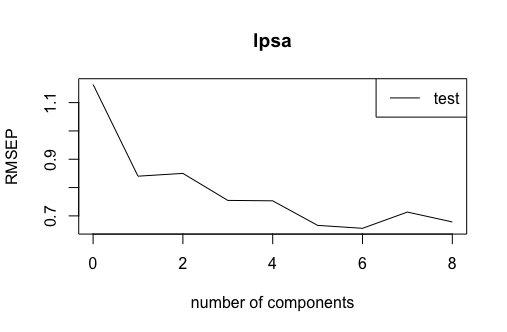
\includegraphics[width=\textwidth]{img/pcr_test.png}
\item For the partial least squares model, the training error v.s. number of principal components and test error v.s number of principal components are shown below. Here, the training data suggests 3  principal components would be best, with 2 and 4-8 components being about as good. The test data also suggests that 3 components would be best. \newline
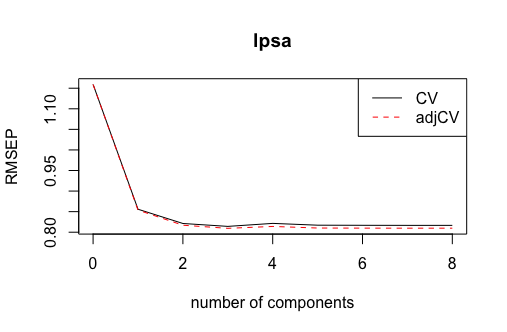
\includegraphics[width=\textwidth]{img/pls_train.png}
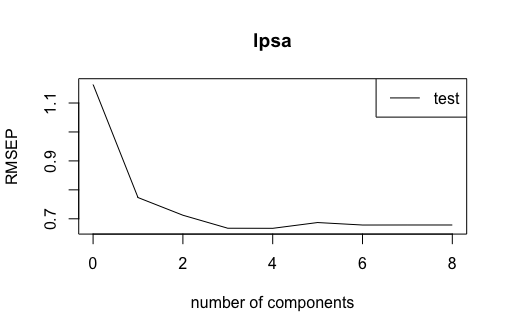
\includegraphics[width=\textwidth]{img/pls_test.png}
\item The visualizations of just the training set then the whole data set for the first for principal components are below. With the addition of the test data the first component clearly appears to capture the separability of the data much better than with just training data alone. \newline
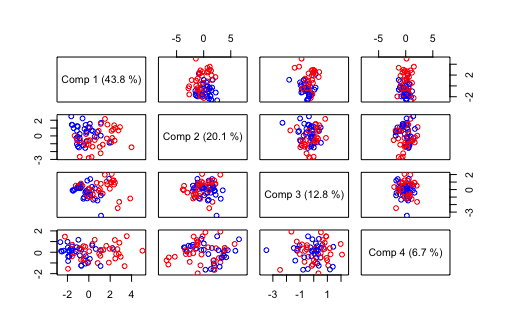
\includegraphics[width=\textwidth]{img/pcr_vis_train.png}
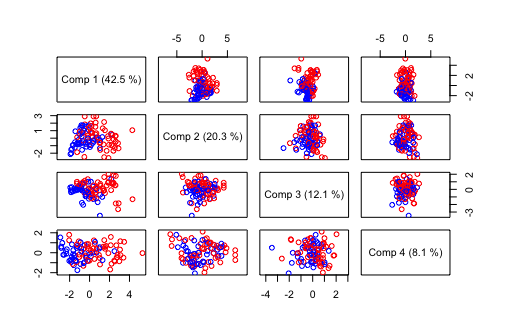
\includegraphics[width=\textwidth]{img/pcr_vis_all.png}
\item The visualizations of just the training set then the whole data set for the first four PLS directions are below. Here both graphs seem to be much more similar to one another, than for PCR. I both cases the first PLS direction seems to accurately capture separability in the data.  \newline
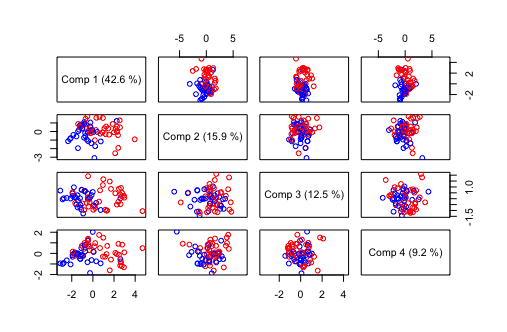
\includegraphics[width=\textwidth]{img/pls_vis_train.png}
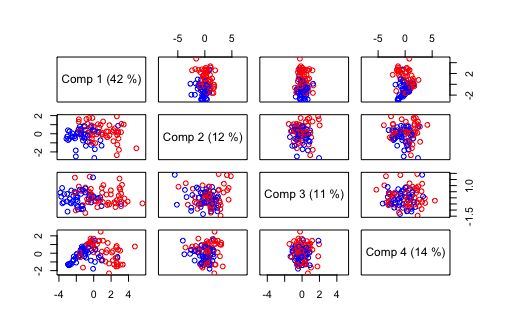
\includegraphics[width=\textwidth]{img/pls_vis_all.png}
\item For PCR, the training and test data suggest very different M values, with little overlap. Here I would chose 8 components. For PLS, the training and test data suggest more similar values for M. This makes sense since PLS is a supervised alternative to PCR that takes into account the response. 
\end{enumerate}